\section{What Grid Computing is}
Grid Computing is a type of Distributed Computing where the resources of many computers, connected by a network, are used in combination to reach a certain common goal.

\begin{figure}[!ht]
    \centering
    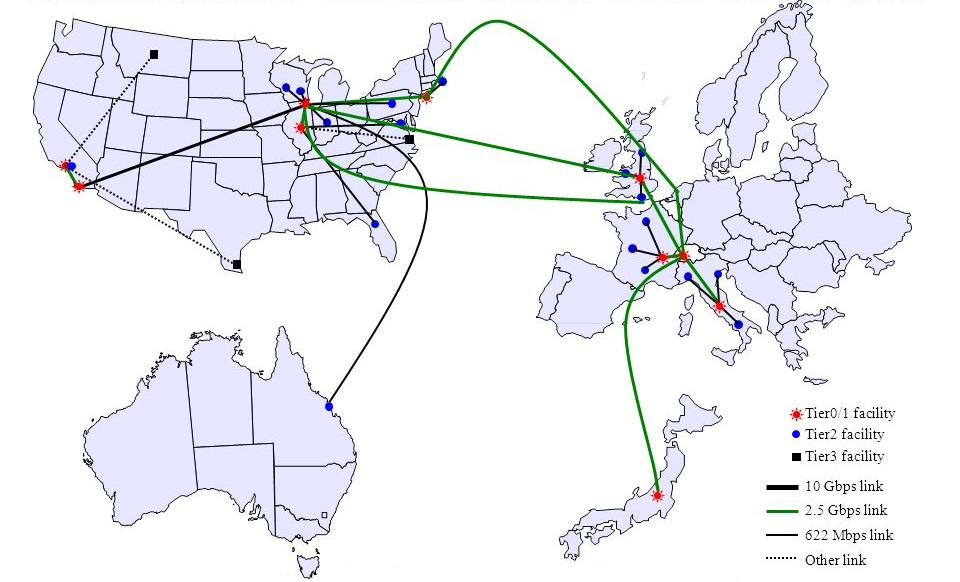
\includegraphics[scale=0.46]{document/chapters/chapter_1/images/iVDGL_globus.jpg}
    \caption{Example of a Grid - iVDGL, the Globus project \cite{iVDGL}}
    \label{fig:iVDGL}
\end{figure}

Compared to traditional Distributed Computing like Cluster Computing, Grid Computing focuses on large-scale resources with geographically dispersed nodes that also tend to be more heterogeneous regarding their hardware and software; this is also due to the fact that while a Cluster is only composed by computers entirely dedicated to perform the tasks requested inside the Cluster (thus coming from an investment and a subsequential setup of the Cluster), a Grid is composed by machines offered mostly on voluntary basis by regular day-to-day users scattered around the planet.

Another important aspect that differentiates Grid Computing from Cluster Computing is how the last one tends to be more focused on a particular task while the Grid is designed to a general-purpose tool.

\vspace{5mm}
\begin{figure}[!ht]
    \centering
    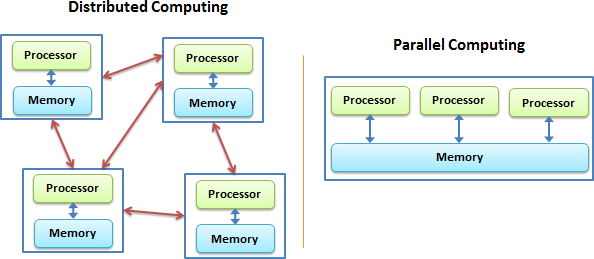
\includegraphics[width=\linewidth]{document/chapters/chapter_1/images/distributed_computing_vs_parallel_computing.png}
    \caption{High-level comparison of Distributed Computing and Parallel Computing \cite{distributed_vs_parallel}}
    \label{fig:distributed_vs_parallel}
\end{figure}
\vspace{2mm}

For certain applications, Grid Computing can be seen as a special type of Parallel Computing that distributes computation among the nodes connected to the Grid utilizing their resources; this approach is in contrast with the traditional notion of a supercomputer, which has many processors connected by a local high-speed bus.
From this difference in approach comes the strength of performing parallel computations in a distributed Grid environment: resources from the machines connected to the Grid can be quickly gathered to perform a task and, after completion, they can be dismantled just as quickly, removing the necessity of maintaining a highly expensive supercomputer; while this is, in a certain way, also true for Cluster Computing, the strength of Grid Computing lies in its ability to reach much greater levels of scalability with relative ease. 

\subsection{The "Grid problem"}
The "Grid problem" is defined as \textit{"flexible, secure and coordinated resource sharing among dynamic collections of individuals, institutions and resources"} \cite{the_anatomy_of_the_grid}
 While being a powerful tool, Grid computing brings with it some inherit challenges that are a byproduct of the flexibility that the grid aims to offer; while designing a Grid system, diverse usage models have to be taken in consideration, ranging from single user to multiuser and from performance sensitive to cost sensitive and hence embracing issues of quality of service, scheduling, co-allocation, resource discovery, security and accounting.
 Quoting a passage from the foundational article \textit{"The anatomy of the Grid: enabling scalable virtual organizations"} by Ian Foster, Carl Kesselman and Steven Tuecke \cite{the_anatomy_of_the_grid}:
\begin{quotation}
    \textit{"The sharing that we are concerned with is not primarily file exchange but rather direct access to computers, software, data and other resources, as is required by a range of collaborative problem-solving and resource-brokering strategies emerging in industry, science and engineering. The sharing is, necessarily, highly controlled, with resources providers and consumers defining clearly and carefully just what is shared, who is allowed to share and the conditions under which sharing occurs."}
\end{quotation}


\subsection{History and applications using the Grid}
Before being referred to as "Grid Computing", the idea of connecting geographically distant computers in order to share resources was known as "Utility Computing"; the term is based on the idea of seeing computing as a public utility, analogous to the phone system. This field was then renamed to "Grid Computing" in the early 1990s, based on the metaphor of making computational power as easy to access as an electric power grid.
Thus, the nomenclature of this technology shifted its focus, representing first the goal of providing public service that could be used by anyone, then an easy-to-scale enabling technology for gathering a vast number of computational resources. In 2007 the term "Cloud Computing", which is conceptually similar to the definition of Grid Computing, came into popularity. Nowadays, Grid Computing is often associated with the delivery of Cloud Computing systems.
\vspace{5mm}

Volunteer computing (having people that voluntarily offer their machines to contribute to a Grid) became relevant first in 1997 with \href{https://www.distributed.net/Main_Page}{distributed.net}, a project that aims to solve mathematical complex and resource-consuming problems using Grid computing; then, in 1999, the \href{https://setiathome.berkeley.edu/}{SETI@home} project used voluntarily offered computers performing distributed computing over a Grid in order to Search for Extraterrestrial Intelligence (hence the acronym "SETI") analyzing radio signals.

TODO other projects and current state